\documentclass{beamer}
\usepackage{../tut-slides}
\usepackage{../mathoperatorsAuD}

\usepackage{csquotes}
\usepackage{cancel}

\usepackage{amsmath,amssymb}

\usepackage{tikz}
\usetikzlibrary{positioning,automata, matrix, trees}
\usetikzlibrary{calc,positioning,backgrounds,arrows.meta}
\usetikzlibrary{patterns,snakes}
\usepackage{forest}


\usepackage{booktabs}
\usepackage{tabularx}
\usepackage{tabu}
\newcommand*\head{\rowfont{\bfseries}}
\newcommand*{\tw}{\rowfont{\ttfamily}}

\renewcommand{\tabularxcolumn}[1]{>{\hspace{0pt}}m{#1}}

\usepackage{listings}
\lstset{ 
	basicstyle=\footnotesize\ttfamily,        % the size of the fonts that are used for the code
	breakatwhitespace=false,         % sets if automatic breaks should only happen at whitespace
	breaklines=true,                 % sets automatic line breaking
	commentstyle=\itshape,    	     % comment style
	escapeinside={\%*}{*)},          % if you want to add LaTeX within your code
	extendedchars=true,              % lets you use non-ASCII characters; for 8-bits encodings only, does not work with UTF-8
	firstnumber=1,                % start line enumeration with line 1000
	frame=none,
	keywordstyle=\bfseries,       % keyword style
	morekeywords={}, 
	language=C,                 % the language of the code
	numbers=left,                    % where to put the line-numbers; possible: (none, left, right)
	numbersep=5pt,                   % how far the line-numbers are from the code
	numberstyle=\tiny\color{cdgray!50}, % the style that is used for the line-numbers
	rulecolor=\color{cddarkblue}, 
	tabsize=2,	                   % sets default tabsize to 2 spaces
}
\lstdefinestyle{am0}{ 
	basicstyle=\footnotesize\ttfamily,        % the size of the fonts that are used for the code
	breakatwhitespace=false,         % sets if automatic breaks should only happen at whitespace
	breaklines=true,                 % sets automatic line breaking
	commentstyle=\color{cdgray},    	     % comment style
	escapeinside={(*@}{@*)},          % if you want to add LaTeX within your code
	extendedchars=true,              % lets you use non-ASCII characters; for 8-bits encodings only, does not work with UTF-8
	firstnumber=1,                % start line enumeration with line 1000
	frame=none,
	keywordstyle=\bfseries,       % keyword style
	morekeywords={READ,LOAD,GT,JMC,STORE,JMP,WRITE}, 
%	language=AM0,                 % the language of the code
	numbers=left,                    % where to put the line-numbers; possible: (none, left, right)
	numbersep=5pt,                   % how far the line-numbers are from the code
	numberstyle=\tiny\ttfamily\color{cdgray!50}, % the style that is used for the line-numbers
	rulecolor=\color{cddarkblue}, 
	tabsize=2,	                   % sets default tabsize to 2 spaces
}


\usepackage{textgreek}


\renewcommand{\emph}[1]{\textbf{#1}}
\newcommand{\coloremph}[1]{\textcolor{cdpurple}{#1}}
\newcommand{\col}[1]{\textcolor{cdpurple}{\boldsymbol{#1}}}
\newcommand{\coll}[1]{\textcolor{cddarkgreen}{\boldsymbol{#1}}}
\newcommand{\colll}[1]{\textcolor{cdorange}{\boldsymbol{#1}}}
%\newcommand{\step}[2][]{\ensuremath{\overset{{#1} (\text{#2})}{=}}}
%\newcommand*{\astep}[2][]{\ensuremath{\overset{{#1} (\text{#2})}&{=}}}

\newcommand{\num}[1]{\ensuremath{\langle #1 \rangle}}

\undef\trans
\DeclareMathOperator{\trans}{trans}

\newcommand{\logand}{ \ \land \ }

\begin{document}	
	\title{Programmierung}
	\subtitle{Übung 12: Hoare-Kalkül}
	\author{Eric Kunze}
	\email{eric.kunze@mailbox.tu-dresden.de}
%	\city{TU Dresden}
	\date{}
%	\institute{Lehrstuhl für Grundlagen der Programmierung}
%	\titlegraphic{
\includegraphics[width=2cm]{../TUD-white.pdf}}
	
	\maketitle
	

%%%%%%%%%%%%%%%%%%%%%%%%%%%%%%%%%%%%%%%%%%%%%%%%%%%%%%%%%%%%%%%%%%%%%%%%%%%%%

\begin{frame}[fragile] \frametitle{Inhalt}
	\begin{enumerate}
		\item Funktionale Programmierung
		\begin{enumerate}
			\item Einführung in Haskell: Listen
			\item Algebraische Datentypen
			\item Funktionen höherer Ordnung
			\item Typpolymorphie \& Unifikation
			\item Beweis von Programmeigenschaften
			\item \textlambda--Kalkül
		\end{enumerate}
		\item Logikprogrammierung
		\item Implementierung einer imperativen Programmiersprache
		\begin{enumerate}
			\item Implementierung von C${}_\text{0}$
			\item Implementierung von C${}_\text{1}$
		\end{enumerate}
		\item \textbf{Verifikation von Programmeigenschaften}
		\item H${}_\text{0}$ -- ein einfacher Kern von Haskell
	\end{enumerate}
\end{frame}



\section{\textsc{Hoare}-Kalkül}

\begin{frame} \frametitle{\textsc{Hoare}-Kalkül}
	\begin{itemize}
		\item Beweis / Verifikation von Programmeigenschaften \pause 
		\item Verifikationsformeln der Form $\{P\} \ \mathbf{A} \ \{Q\}$
		\begin{itemize}
			\item $P$ und $Q$ sind Zusicherungen (prädikatenlogische Ausdrücke)
			\item $P$ heißt \emph{Vorbedingung}, $Q$ heißt \emph{Nachbedingung}
			\item Beschreibung der Veränderung von Zusicherungen \pause
			\item \emph{Bedeutung}: Wenn die Variablenwerte vor Ausführung von $\mathbf{A}$ die Zusicherung $P$ erfüllen und $\mathbf{A}$ terminiert, dann erfüllen die Variablen nach Ausführung von $\mathbf{A}$ die Zusicherung $Q$
		\end{itemize} \pause
		\item Aufstellen eines Beweisbaumes mit zur Verfügung stehenden Regeln
	\end{itemize}
\end{frame}


\begin{frame} \frametitle{\textsc{Hoare}-Kalkül -- Regeln}
	\begin{itemize}
		\item Zuweisungsaxiom
		\item Sequenzregel
		\item CompRegel
		\item Iterationsregel
		\item (erste und zweite) Alternativregel
		\item Konsequenzregeln
		\begin{itemize}
			\item stärkere Vorbedingung
			\item schwächere Nachbedingung
		\end{itemize}
	\end{itemize}
\end{frame}

\begin{frame} \frametitle{Schleifeninvariante}
	Für die Iterationsregel benötigen wir die Schleifeninvariante $SI$.
	In den meisten unserer Fälle ist diese von der Form $SI = A \land B$, wobei
	\begin{itemize}
		\item $A$ den Zusammenhang zwischen Zählvariable und Akkumulationsvariablen beschreibt. Führe dazu einige Iterationen der Schleife durch und leite daraus einen Zusammenhang her.
		\item $B$ die abgeschwächte Schleifenbedingung ist. Dabei nehmen wir die letztmögliche Variablenbelegung, für die die Schleifenbedingung $\pi$ noch wahr ist und führen den Schleifenrumpf noch einmal darauf aus ($\to \pi'$). \\
		$\Rightarrow B = \pi \cup \pi'$
	\end{itemize}
\end{frame}



\section{Aufgabe 1}

\begin{frame} \frametitle{Aufgabe 1 -- Teil (a)}
	
	\textbf{Verfikationsformel:}
	\begin{tiny}
		\begin{equation*}
			\underbrace{\{ (\texttt{x} \ge 0) \land (\texttt{x} = \texttt{x1}) \land (\texttt{z}=0) \land (\texttt{y} \ge 0) \}}_{\text{Vorbedingung}} \ \ \texttt{\emph{while} (\texttt{x1} > 0) \{\texttt{x1 = x1-1}; \texttt{z} = \texttt{z} + \texttt{y};\}} \ \ \underbrace{\{(\texttt{z} = \texttt{y} * \texttt{x})\}}_{\text{Nachbedingung}}
		\end{equation*}
	\end{tiny}
	
	
	\pause
	
	\textbf{Schleifeninvariante:} $\qquad$ $SI = A \land B$ \pause
	
	\begin{minipage}{\dimexpr0.5\linewidth-\fboxrule-\fboxsep}
		\begin{center}
			\begin{tabu}{ccc}
				\toprule
				\head $\#$ & \texttt{x1} & \texttt{z} \\
				\midrule \midrule
				$0$	 & $x$   & $0$  \\
				$1$  & $x-1$ & $y$  \\
				$2$  & $x-2$ & $2y$ \\
				$N$  & $x-N$ & $Ny$ \\
				\bottomrule
			\end{tabu}
		\end{center}
	\end{minipage}
	\begin{minipage}{\dimexpr0.5\linewidth-\fboxrule-\fboxsep}
		Als Gleichungssystem:
		\begin{equation*}
			\begin{array}{rl}
			\texttt{x1} &\texttt{= x - N} \\ \texttt{z} &\texttt{= N * y}
			\end{array}
		\end{equation*}
		$\Rightarrow \enskip A = (\texttt{z = (x-x1) * y})$		
	\end{minipage}
\end{frame}

\begin{frame} \frametitle{Aufgabe 1 -- Teil (a)}
	\fbox{$SI = A \land B$} und wir wissen schon $A = (\texttt{z = (x-x1) * y})$
	
	\bigskip
	
	\textbf{abgeschwächte Schleifenbedingung:}
	\begin{itemize}
		\item Schleifenbedingung: $\pi = (\texttt{x1 > 0})$
		\item Schleifenbedingung letztmalig wahr für \texttt{x1 = 1}
		\item Wert nach nochmaligem Schleifendurchlauf: $\pi' = (\texttt{x1 = 0})$
		\item $B = \pi \cup \pi' = (\texttt{x1} \ge \texttt{0})$ \hspace{1cm} {\footnotesize \itshape (symbolische Schreibweise)}
	\end{itemize}
	\medskip
	
	\fbox{$\Longrightarrow SI = A \land B = (\texttt{z = (x-x1) * y}) \land (\texttt{x1} \ge \texttt{0})$}
\end{frame}


\begin{frame} \frametitle{Aufgabe 1 -- Teil (b)}
	\small
	
	\begin{center}
		\emph{Verfikationsformel:} \tiny
		\begin{equation*}
			\{ (x \ge 0) \land (x = x1) \land (z=0) \land (y \ge 0) \} \ \ \texttt{\emph{while} (x1 > 0) \{x1 = x1-1; z = z+y;\}} \ \ \{(z = y*x)\}
		\end{equation*}
	\end{center}
	
	\bigskip \pause
	
	Sei $SI = A \land B = (\texttt{z=(x-x1)*y}) \land (\texttt{x1} \ge \texttt{0})$ und $\pi = (\texttt{x1 > 0})$.
	
	
	\begin{align*}
		A &= C = D = G = SI \\
		B &= SI \land \lnot \pi = (\texttt{z=(x-x1)*y}) \land (\texttt{x1} \ge \texttt{0}) \land \lnot (\texttt{x1 > 0}) \\
		E &= SI \land \pi = (\texttt{z=(x-x1)*y}) \land (\texttt{x1} \ge \texttt{0}) \land (\texttt{x1 > 0} )
	\end{align*}
\end{frame}


\begin{frame} \frametitle{Aufgabe 1 -- Teil (c)}
	\begin{center}
		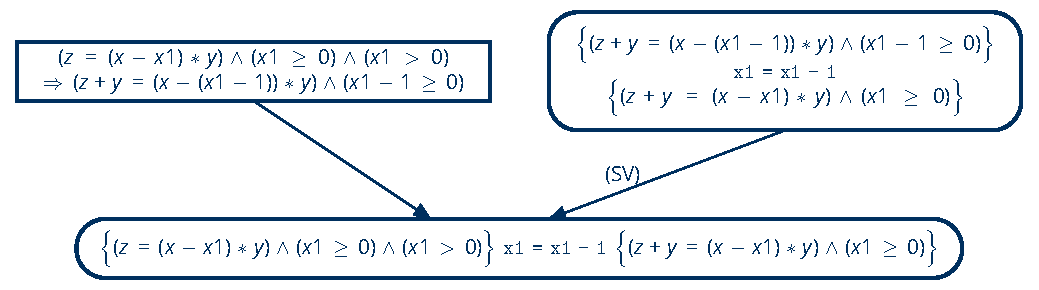
\includegraphics[width=\linewidth]{tut12-abb}
	\end{center}
	wobei (beachte: $x1$ ist Ganzzahl)
	\begin{align*}
		&(z = (x - x1) * y) \land (x1 \ge 0) \land (x1 > 0) \\
		\Leftrightarrow \enskip &(z + y = (x - x1) * y + y) \land (x1 \ge 0) \land (x1 > 0) \\
		\Leftrightarrow \enskip &(z + y = (x - x1 + 1) * y) \land (x1 \ge 0) \land (x1 > 0) \\
		\Leftrightarrow \enskip &(z + y = (x - (x1 - 1)) * y) \land (x1 \ge 0) \land (x1 > 0) \\
		\Leftrightarrow \enskip &(z + y = (x - (x1 - 1)) * y) \land (x1 \ge 0) \land (x1 - 1 \ge 0)
	\end{align*}
\end{frame}

\section{Aufgabe 2}

\begin{frame} \frametitle{Aufgabe 2 -- Teil (a)}
	\begin{minipage}{\dimexpr0.5\linewidth-\fboxrule-\fboxsep}
		\begin{align*}
			A &= \text{true} \logand (y < 0) \\
			B &= \text{true} \logand \lnot \ (y < 0) \\
			C &= A \\
			D &= A \\
			E &= ( -(3*y) + 1 \ge 0) \\
			F &= E 
		\end{align*}
	\end{minipage}
	\begin{minipage}{\dimexpr0.5\linewidth-\fboxrule-\fboxsep}
		\begin{align*}
		G &= E \\
		H &= (-x + 1 \ge 0) \\
		J &= H \\
		K &= (y \ge 0) \\
		L &= \text{stärkere Vorbedingung} \\
		M &= \text{Sequenzregel} 
		\end{align*}
	\end{minipage}	
\end{frame}

\begin{frame} \frametitle{Aufgabe 2 -- Teil (b)}
	\begin{center}
		\textbf{zu zeigen:} $\text{true} \ \land \ (y < 0) \enskip \Rightarrow \enskip (-3 * y + 1 \ge 0)$
		\pause
		\begin{alignat*}{2}
			\text{true} \ \land \ (y < 0) \enskip &\Rightarrow \quad &y &< 0 \\
			&\Rightarrow \quad &-3 * y &> 0 \\ 
			&\Rightarrow \quad &-3 * y + 1 &> 1 \\ 
			&\Rightarrow \quad &-3 * y + 1 &\ge 0 
		\end{alignat*}
	\end{center}
\end{frame}

\end{document}

